\documentclass[10pt,a4paper]{article}
\usepackage[T1]{fontenc}
\usepackage{amsmath}
\usepackage{amsfonts}
\usepackage{amssymb}
\usepackage{graphicx}
\usepackage{enumitem}
\usepackage{titlesec}
\usepackage{geometry}
\geometry{a4paper, margin=1in}
\usepackage{hyperref}
\usepackage[portuguese]{babel}

% Configurações de títulos para um visual mais limpo e profissional
\titleformat{\section}[block]{\bfseries\Large\raggedright}{}{0em}{}
\titlespacing{\section}{0pt}{1.5em}{1em}

\title{Plano de Formação: Linux - Serviços de Redes}
\author{Formador: [Seu Nome]}
\date{Data de Elaboração: [Data]}


\begin{document}
	
	\section*{Conteúdos}
	
	\subsection*{0. Introdução a Fundamentos de Redes (10 horas)}
	\vspace{-1.2em}
	\paragraph{}
	Antes de explorarmos os serviços de rede, é fundamental entender a base: os endereços IP e a comunicação na rede.
	
	\begin{itemize}
		\item \textbf{Endereços IP e Máscaras de Rede} (4 horas) \\
		Explicação dos endereços IPv4 (Classes A, B, C) e IPv6, e como as máscaras de rede definem a sub-rede.
		\begin{verbatim}
			# Exemplo de IP e máscara
			Endereço IP: 192.168.1.50
			Máscara de Rede: 255.255.255.0  (ou /24)
		\end{verbatim}
		
		\item \textbf{Ferramentas de Diagnóstico de Rede} (3 horas) \\
		Apresentar ferramentas essenciais para testar a conectividade.
		\begin{verbatim}
			ping google.com          # Testar a conectividade com um host
			traceroute google.com    # Seguir o caminho até um destino
			ifconfig / ip addr       # Ver os detalhes das interfaces de rede
		\end{verbatim}
		
		\item \textbf{Exercício de Consolidação} (3 horas) \\
		1. Abra o terminal e use `ifconfig` ou `ip addr` para encontrar o endereço IP da sua máquina.
		2. Use o comando `ping` para testar a conectividade com o router da rede (geralmente 192.168.1.1 ou 10.0.0.1).
		3. Use o `traceroute` para seguir o caminho até um site conhecido e explique o que vê em cada "salto".
	\end{itemize}
	
	---
	
	\subsection*{1. Serviços de rede (15 horas)}
	\vspace{-1.2em}
	\paragraph{}
	Nesta secção, vamos explorar como os serviços de rede são geridos no Linux, desde o seu início até ao encerramento, e os principais ficheiros e diretórios envolvidos neste processo.
	
	\begin{itemize}
		\item \textbf{O Gestor de Tarefas: O Papel do \texttt{systemd}} (3 horas) \\
		Pense no \texttt{systemd} como o "gerente de todas as tarefas" do seu computador. Ele garante que tudo comece a funcionar na ordem certa quando o sistema é ligado.
		
		\item \textbf{Controlar Serviços com \texttt{systemctl}} (5 horas) \\
		O comando \texttt{systemctl} é como a "lista de comandos" para o gestor de tarefas.
		\begin{verbatim}
			# Ver o estado de um serviço (Exemplo: SSH)
			systemctl status sshd
			
			# Ligar, desligar e reiniciar um serviço
			systemctl start sshd
			systemctl stop sshd
			systemctl restart sshd
		\end{verbatim}
		
		\begin{figure}[h]
			\centering
			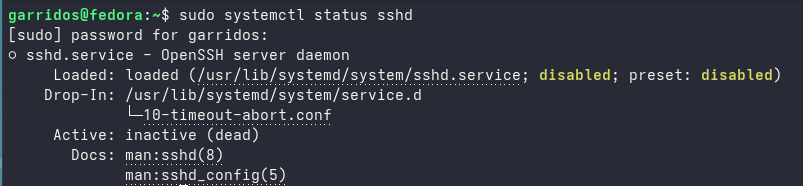
\includegraphics[width=0.8\textwidth]{img/systemctl_status.png}
			\caption{Exemplo da saída do comando \texttt{systemctl status sshd}. \textit{Fonte: Imagem encontrada via Google Images.}}
			\label{fig:systemctl_status}
		\end{figure}
		
		\item \textbf{Tarefas Programadas e Serviços On-Demand} (5 horas) \\
		Aprofundar o uso do \texttt{systemd} para além da gestão básica de serviços.
		\begin{itemize}
			\item \textbf{Systemd Timers}: Uma alternativa moderna ao `cron` para agendar tarefas.
			\item \textbf{Systemd Sockets}: Iniciar serviços "on-demand" apenas quando há tráfego numa porta específica.
		\end{itemize}
		
		\item \textbf{Exercício de Consolidação} (2 horas)
		1. Crie uma unidade de serviço (`.service`) e uma unidade de temporizador (`.timer`) para um script simples que escreve a data e hora num ficheiro a cada minuto.
		2. Verifique o estado do temporizador e do serviço com \texttt{systemctl list-timers}.
	\end{itemize}
	
	---
	
	\subsection*{2. XINET.d (5 horas)}
	\vspace{-1.2em}
	\paragraph{}
	O \texttt{xinetd} é como um "rececionista" que só acorda um funcionário (serviço) quando alguém aparece para o ver.
	
	\begin{itemize}
		\item \textbf{Configuração e Gestão} (3 horas) \\
		As configurações do \texttt{xinetd} estão nos ficheiros do diretório \texttt{/etc/xinet.d/}. Cada serviço tem o seu próprio "cartão de identificação" com opções como \texttt{server}, \texttt{port} e \texttt{disable}.
		
		\item \textbf{Exercício de Consolidação} (2 horas) \\
		1. Encontre o ficheiro de configuração do serviço \texttt{ftp} no diretório \texttt{/etc/xinet.d/}.
		2. Altere o valor da opção \texttt{disable} para habilitá-lo.
		3. Crie uma nova configuração para um serviço simples, como um servidor de eco, e verifique o seu funcionamento.
	\end{itemize}
	
	---
	
	\subsection*{3. TCPWrappers (5 horas)}
	\vspace{-1.2em}
	\paragraph{}
	Pense nos \texttt{TCPWrappers} como um porteiro. Ele decide quem pode entrar (permitir) e quem não pode (negar) num serviço, com base no endereço IP.
	
	\begin{itemize}
		\item \textbf{As Duas Listas: `hosts.allow` e `hosts.deny`} (2 horas) \\
		- \texttt{hosts.allow}: A "lista de convidados". Se alguém estiver aqui, entra.
		- \texttt{hosts.deny}: A "lista negra". Se alguém não estiver na lista de convidados e estiver aqui, é barrado.
		
		\item \textbf{Sintaxe e Exemplos Avançados} (2 horas) \\
		Pode usar `ALL` para todos e `EXCEPT` para criar exceções.
		\begin{verbatim}
			# No ficheiro /etc/hosts.allow
			sshd: 192.168.1.100 EXCEPT 192.168.1.101
		\end{verbatim}
		
		\item \textbf{Exercício de Consolidação} (1 hora) \\
		1. Configure o seu ficheiro \texttt{hosts.deny} para negar o acesso SSH a todos.
		2. No ficheiro \texttt{hosts.allow}, adicione o IP do seu computador para poder aceder.
	\end{itemize}
	
	---
	
	\subsection*{4. NIS (10 horas)}
	\vspace{-1.2em}
	\paragraph{}
	O NIS é como ter uma única "identidade" para toda uma rede de computadores. Em vez de ter uma conta de utilizador em cada máquina, você tem uma conta num servidor central que funciona em todas as máquinas NIS.
	
	\begin{itemize}
		\item \textbf{Arquitetura NIS (Servidor Mestre e Cliente)} (3 horas) \\
		- \textbf{Servidor Mestre}: Tem a lista principal de utilizadores e grupos.
		- \textbf{Cliente NIS}: Pede ao servidor as informações de utilizadores. O `ypbind` é o serviço que o cliente usa para encontrar o servidor.
		
		\item \textbf{Configuração de um Servidor NIS Mestre} (5 horas) \\
		Passos detalhados para instalar o `ypserv` e configurar os mapas NIS (`/etc/passwd`, `/etc/group`, etc.) e exportá-los para os clientes.
		
		\item \textbf{Exercício de Consolidação} (2 horas) \\
		1. Numa máquina cliente, use o comando \texttt{ypwhich} para ver qual é o servidor NIS.
		2. Use \texttt{ypcat passwd} para listar as contas de utilizador.
		3. Crie uma nova conta no servidor NIS e verifique se consegue iniciar sessão com essa conta a partir do computador cliente.
	\end{itemize}
	
	---
	
	\subsection*{5. DHCP (15 horas)}
	\vspace{-1.2em}
	\paragraph{}
	O DHCP é um protocolo que automaticamente dá um "endereço de rua" (o endereço IP) a cada dispositivo que se liga à sua rede.
	
	\begin{itemize}
		\item \textbf{O Processo DORA: Como funciona?} (4 horas) \\
		Pense no processo DORA como uma conversa entre um novo dispositivo e o servidor DHCP:
		\begin{enumerate}
			\item **D**iscover: "Olá, estou aqui! Há algum servidor DHCP disponível?"
			\item **O**ffer: "Sim, eu sou um servidor! Aqui está um endereço IP que pode usar."
			\item **R**equest: "OK, obrigado! Quero usar este endereço."
			\item **A**cknowledge: "Certo, é todo seu! Divirta-se na rede!"
		\end{enumerate}
		
		\begin{figure}[h]
			\centering
			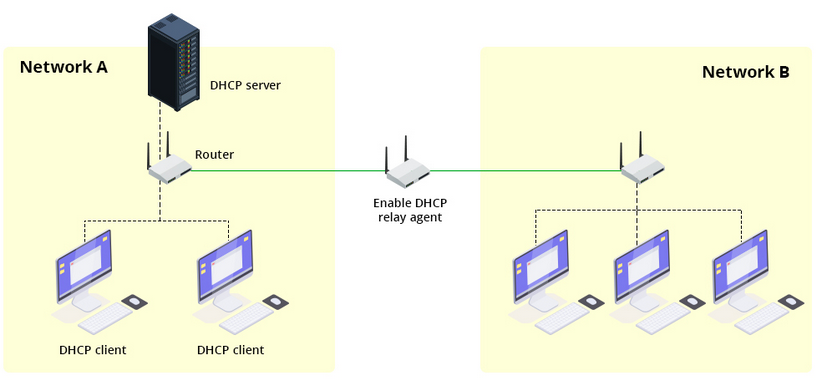
\includegraphics[width=0.8\textwidth]{img/dhcp_dora.png}
			\caption{Diagrama do processo DORA. \textit{Fonte: Imagem encontrada via Google Images.}}
			\label{fig:dhcp_dora}
		\end{figure}
		
		\item \textbf{Configuração e Atribuição de Endereços} (7 horas) \\
		Aprofundar a configuração do servidor DHCP no ficheiro \texttt{dhcpd.conf}.
		- \texttt{subnet}: Define a rede que o servidor vai gerir.
		- \texttt{range}: A lista de IPs que serão atribuídos dinamicamente.
		- \texttt{option routers}: Define o endereço do router/gateway.
		- \texttt{host}: Para dar um IP fixo a um computador específico (com base no endereço MAC).
		
		\item \textbf{Conceitos Avançados: DHCP Relay Agent} (2 horas) \\
		Explicar como um **DHCP Relay Agent** pode ser usado para encaminhar pedidos de DHCP entre redes, eliminando a necessidade de ter um servidor DHCP em cada sub-rede.
		
		\item \textbf{Exercício de Consolidação} (2 horas) \\
		1. Configure um servidor DHCP para a sua rede de treino com um `range` de IPs dinâmicos.
		2. Adicione uma entrada estática para o computador do instrutor.
		3. Configure um cliente Linux para obter o IP do servidor e verifique se as configurações (IP, gateway, DNS) estão corretas.
	\end{itemize}
	
	---
	
	\subsection*{6. DNS (20 horas)}
	\vspace{-1.2em}
	\paragraph{}
	O DNS é como a "lista telefónica" da internet. Ele traduz nomes fáceis de lembrar (como `google.com`) em endereços IP que os computadores entendem.
	
	\begin{itemize}
		\item \textbf{Como a Lista Telefónica Funciona: A Hierarquia} (6 horas) \\
		A consulta de DNS é um processo de "perguntas e respostas" entre o cliente, o servidor DNS local e a hierarquia de servidores de raiz, TLD e autoritativos.
		
		\begin{figure}[h]
			\centering
			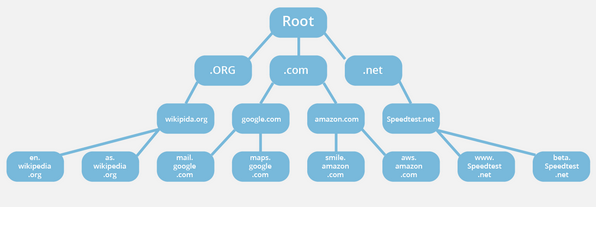
\includegraphics[width=0.8\textwidth]{img/dns_lookup.png}
			\caption{Fluxo de uma consulta DNS típica, mostrando a hierarquia de servidores. \textit{Fonte: Imagem encontrada via Google Images.}}
			\label{fig:dns_lookup}
		\end{figure}
		
		\item \textbf{Tipos de Registos DNS (A, AAAA, CNAME, MX, PTR)} (4 horas) \\
		- \texttt{A}: Mapeia um nome de domínio para um endereço IPv4.
		- \texttt{CNAME}: Cria um "apelido" para outro nome de domínio.
		- \texttt{MX}: Especifica o servidor de correio para um domínio.
		- \texttt{PTR}: Usado para a pesquisa inversa, mapeando um IP para um nome de domínio.
		
		\item \textbf{Configuração de um Servidor DNS com BIND} (8 horas) \\
		Instalar o `BIND` (servidor DNS mais popular) e configurar um servidor DNS primário (autoritativo) para um domínio.
		- Configurar o ficheiro de zona de **`forward lookup`** para traduzir nomes para IPs.
		- Configurar o ficheiro de zona de **`reverse lookup`** para traduzir IPs para nomes.
		
		\item \textbf{Exercício de Consolidação} (2 horas) \\
		1. Crie um servidor DNS com o BIND e configure-o para ser autoritativo para um domínio fictício (`meu-curso.com`).
		2. Adicione vários registos (A, CNAME) para máquinas na sua rede.
		3. Configure uma máquina cliente para usar este novo servidor DNS e use o `dig` para testar se as consultas estão a funcionar.
	\end{itemize}
	
	---
	
	\subsection*{7. LOGS (10 horas)}
	\vspace{-1.2em}
	\paragraph{}
	Os logs são como um "diário de bordo" do seu computador. Eles registam tudo o que acontece e são essenciais para encontrar erros e problemas.
	
	\begin{itemize}
		\item \textbf{Onde Encontrar o Diário} (2 horas) \\
		A maioria dos logs está em \texttt{/var/log}. Os ficheiros mais importantes são:
		- \texttt{syslog} ou \texttt{messages}: Mensagens gerais do sistema.
		- \texttt{auth.log}: Registos de login e autenticação.
		
		\item \textbf{Como Ler o Diário: Comandos Úteis} (3 horas) \\
		- \texttt{tail -f /var/log/syslog}: Mostra as últimas linhas do ficheiro e acompanha as novas linhas em tempo real.
		- \texttt{grep "erro" /var/log/syslog}: Procura por uma palavra-chave como "erro".
		
		\item \textbf{Gerir o Diário: Rotação de Logs (`logrotate`)} (3 horas) \\
		Explicar o conceito de rotação de logs para evitar que os ficheiros fiquem demasiado grandes, e como configurar o `logrotate`.
		
		\item \textbf{Logging Centralizado} (2 horas) \\
		Introdução ao conceito de enviar logs de várias máquinas para um servidor central, o que facilita a gestão e a monitorização de redes maiores, usando ferramentas como o `syslog-ng` ou `rsyslog`.
		
	\end{itemize}
	
\end{document}